\documentclass{article} % 定义文档类型为文章
\usepackage{pgfplots} % 导入pgfplots包，用于创建图表
\pgfplotsset{compat=1.18} % 设置pgfplots的兼容性版本

\begin{document}

\section*{Model Comparison using Grouped Bar Chart} % 章节标题，描述图表内容

\begin{figure}[h!] % 浮动图形环境，h!表示尽可能在当前位置显示
    \centering % 居中图形
    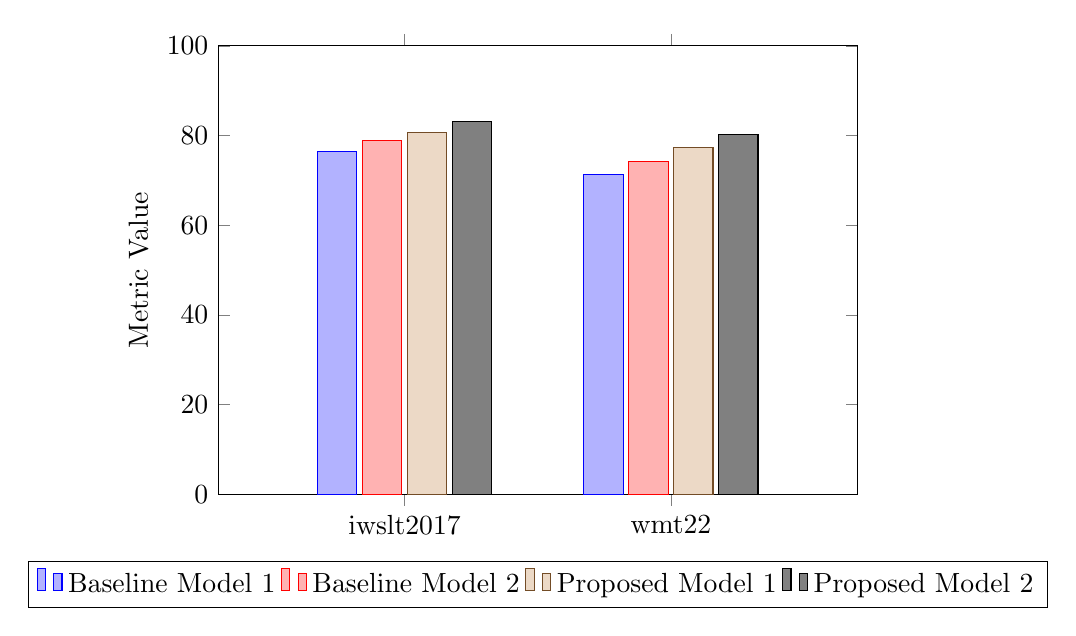
\begin{tikzpicture} % 开始TikZ画图环境
        \begin{axis}[ % 开始axis环境，设置图表参数
            ybar, % 垂直条形图
            bar width=.5cm, % 设置条形宽度
            enlarge x limits=0.7, % 增加x轴显示范围
            legend style={ % 设置图例样式
                at={(0.5,-0.15)}, % 图例位置在图表下方，水平居中
                anchor=north, % 图例锚点在上方
                legend columns=-1 % 图例列数，-1表示自动计算
            },
            ylabel={Metric Value}, % y轴标签
            symbolic x coords={iwslt2017, wmt22}, % 设置x轴坐标为象征性坐标
            xtick=data, % x轴刻度与数据点对齐
            %nodes near coords, % 在每个条形旁边显示数值
            ymin=0, ymax=100, % 设置y轴范围，根据数据调整
            width=0.8\textwidth, % 图表宽度
            height=0.6\textwidth % 图表高度
        ]
        % 添加条形图数据，使用提供的数据替换
        \addplot coordinates {(iwslt2017,76.42141589) (wmt22,71.26040225)};
        \addplot coordinates {(iwslt2017,78.92049729) (wmt22,74.20203974)};
        \addplot coordinates {(iwslt2017,80.7341152) (wmt22,77.29298931)};
        \addplot coordinates {(iwslt2017,83.04977006) (wmt22,80.26201353)};
        % 设置图例条目
        \legend{Baseline Model 1, Baseline Model 2, Proposed Model 1, Proposed Model 2}
        \end{axis}
    \end{tikzpicture}
    % 设置图表标题
    \caption{Grouped Bar Chart comparing four models across two metrics (IWSLT2017 and WMT22)}
\end{figure}

\end{document}